\documentclass[10pt]{book}

\usepackage[T1]{fontenc}
\usepackage[utf8]{inputenc}
\usepackage[english]{babel}
\usepackage{geometry}
\usepackage{graphicx}
\usepackage[pdfa=true]{hyperref}
\usepackage{cite}
\usepackage{listings}
\usepackage[printonlyused,withpage]{acronym}
\usepackage{siunitx}
\usepackage{multirow}
\usepackage{setspace}
\usepackage{xcolor}
\usepackage{listings}
\usepackage{tabularx}
\usepackage{marvosym}

% OWN packages
\usepackage{wrapfig}
\usepackage{cleveref}

%--- pdf/a format ----
% insert metadata about the document here
\RequirePackage{filecontents}
\begin{filecontents*}{\jobname.xmpdata}
\Title{Bachelor thesis}
\Author{Robin William hundt}
\Language{en-US}
\Subject{The abstract, or short description.}
\Keywords{keyword1\sep keyword2\sep keyword3}
\end{filecontents*}
\usepackage{colorprofiles}
\usepackage[a-1b,mathxmp]{pdfx}[2018/12/22]
\usepackage[T1]{fontenc}
\hypersetup{pdfstartview=}


%
% This is the official thesis template of
% the Institute of Computer Science at the
% Georg-August-University of Göttingen
%
%      author: kellner@cs.uni-goettingen.de
% last update: 17/02/2015
%
% If you find any sort of mistake please let me know
% so that it can be fixed in future releases.
%


%--- include custom commands ---
\input{common/commands}

%--- include general configuration ---
\input{common/config}


%--- basic document configuration ---
\newcommand{\mytype}{Bachelor's Thesis}
%\newcommand{\mytype}{Master's Thesis}

\newcommand{\mycourse}{Applied Computer Science}
%\newcommand{\mycourse}{Internet Technologies and Information Systems}

\newcommand{\mytitle}{My Title}
\newcommand{\myauthor}{Robin William Hundt}
\newcommand{\mydepartment}{Institute of Computer Science}
\newcommand{\mysubmissiondate}{09. May 2020}
\newcommand{\mythesisid}{201x-xx} %assigned by examination office
\newcommand{\myfirstsupervisor}{Prof. Dr. Burkhard Morgenstern}
\newcommand{\mysecondsupervisor}{Dr. Peter Meinicke}


\begin{document}

 \pagenumbering{roman}
    \setcounter{page}{1}

   %--- cover page ---
   \input{content/coverpage}
   \myemptypage

    %--- statement page ---
    \input{content/statement}
    \myemptypage

    %--- abstract ---
    \clearpage\phantomsection\pdfbookmark{\abstractname}{abstract}
    \thispagestyle{empty}
    \begin{abstract}
    \textbf{Motivation}\\
    The amount of sequencing data that is generated is ever increasing. A multiple alignment of these sequences is a NP-complete problem, but constitutes an indispensable part of biology and bioinformatics research. Thus, the need for new heuristics and algorithms able to produce biologically plausible multiple sequence alignments with constrained time and memory resources arises.\\
    In the space of alignment-free sequence comparisons, the concept of Spaced Word Matches proved to be a useful tool for the phylogeny reconstruction of large inputs in a fraction of the time and memory a traditional approach would necessitate. In prior work we established that these Spaced Word Matches can be seen as micro-alignments of segments in the input sequences and that it may be possible to efficiently compute a complete alignment by finding and greedily constructing a consistent set of micro-alignments. The aim of this thesis was to further refine, implement and evaluate this alignment approach, in order to answer the question of whether it is possible to \textbf{efficiently} compute \textbf{biologically plausible} multiple sequence alignments by greedily aligning spaced word matches.

    
    \textbf{Results}\\
    This thesis provides an alignment tool called SpaM-Align, referring to \textbf{S}paced \textbf{M}atches, which is based on the idea of greedily aligning spaced word matches. A crucial part SpaM-Align is a reimplementation and improvement upon GABIOS-LIB, a library providing the EdgeAddition algorithm for the incremental computation of a transitive closure of an alignment graph.\\
    The tool is evaluated on the \bb version 3 database and compared to Mafft and Dialign, two established alignment programs. I demonstrate that this approach is able to produce alignments orders of magnitude faster than the Dialign (version 2.2) alignment program, which served as an inspiration for SpaM-Align, and in similar time as the state-of-the-art alignment program Mafft (version 7). However the quality of the produced alignments is, in the best case, slightly worse than those produced by Dialign and significantly worse than what is computed by Mafft.
    
    
\end{abstract}


% TODO maybe structure it with the following headings

%Background: Latest information on the topic; key phrases that pique interest (e.g., “…the role of this enzyme has never been clearly understood”).
%Objective: Your goals; what the study examined and why.
%Methods: Brief description of the study (e.g., retrospective study).
%Results: Findings and observations.
%Conclusions: Were these results expected? Whether more research is needed or not?


    \myemptypage

    %reset acronyms after abstract
    \acresetall

    %--- table of contents ---
    \clearpage\phantomsection\pdfbookmark{\contentsname}{toc}
    \tableofcontents
    \myemptypage

    %--- list of figures ---
    %\listoffigures
    %\myemptypage

    %--- list of tables ---
    %\listoftables
    %\myemptypage

    %--- list of listings ---
    %\lstlistoflistings
    %\myemptypage

    %--- list of acronyms ---
    %\chapter*{List of Abbreviations}

\begin{acronym}[myacronyms]
    \acro{FYI}{For Your Information}    
\end{acronym}

    %\myemptypage


    %arabic page numbers
    \pagenumbering{arabic}
    \setcounter{page}{1}
    
    %--- chaper 1..n ---
    \chapter{Introduction}


\begin{itemize}
	\item maybe show spamograms from \cite{hundt2020praktkium} here which show that high scoring spaced word matches are very likely to be correct as motivation
\end{itemize}
    \myemptypage

    \chapter{Basics}

\section{Multiple sequence alignment}


    \myemptypage

    \chapter{Prior Work}


\section{Gabios-Lib}

\section{Dialign}

\section{Spaced Word Matches}

\subsection{Multi dimensional matches}
	\myemptypage

    \chapter{Algorithm}
\label{chap:algorithm}
This thesis provides an implementation and improvement of the alignment algorithm proposed in \cite{hundt2020praktkium}. It shares the idea of finding segment pairs, or micro alignments, in the input sequences which are greedily aligned with Dialign. However in contrast to that approach, these micro alignments are found by searching for spaced word matches with multiple patterns, a process that is much faster than doing a pairwise alignment for all input sequence combinations. 
\begin{itemize}
	\item describe how micro alignments, especially multi dim are found?
	\item what scoring function should be used and why?
	\item TODO maybe have a look at overlap weight again
	\item describe version of algorithm utilizing eq classes and property described in \ref{fig:unnecessary-cmp} -> should this include data structures and memory evincemanagement?
	\item maybe first dp algorithm without unnecessary cmps (like in Fi. 4 of \cite{abdeddaim1997incremental}) and the formulate with eq classes (which wasn't done in paper) 
	\item highlight how this differs from most alignment algorithms in that it is completely greedy
\end{itemize}

% TODO the algorithms input and output data needs
% to be cleaned up

\begin{algorithm}[h]
	\DontPrintSemicolon
	\KwData{Sequences $S = {S_1, ..., S_N}$}
	\KwData{Pattern set $P = {P_1, ..., P_M}$}
	\KwResult{Partial Alignment $A$ }
	\SetKwFunction{sort}{sort\_by\_score\_descending}
	\SetKwFunction{incons}{is\_inconsistent}
	\SetKwFunction{findspam}{find\_spaced\_word\_matches}
	\SetKwFunction{addsite}{add\_site\_pair}
	\SetKwFunction{notaligned}{not\_aligned}
	
	
	$A \leftarrow$ $\{\}$\;
	
	micro\_alignments $\leftarrow$ \findspam{$S$, $P$}\;
	micro\_alignments.\sort{}\;
	
	\ForEach{ma in micro\_alignments}{
		\If{\incons{ma, $A$}}{
			continue\;
		}
		\ForEach{site\_pair in ma}{
		\If{$A$.\notaligned{site\_pair}} {
				$A$.\addsite{site\_pair}\;	
			}
		}
	}	
	\Return $A$\;
	
	\caption{\bf{align($S$, $P$)}}
	\label{alg:align}
\end{algorithm}

TODO: describe find\_spaced\_word\_matches

The, unfortunately incomplete, description of the \textit{EdgeAddition} algorithm in \cite{abdeddaim2000speeding} lead to the proposal of the algorithm \ref{alg:add-site-pair} in the preliminary work \cite{hundt2020praktkium}; due to the incomplete understanding it is computationally much more expensive than necessary since for every site pair that is added, many sites are considered whose transitivity frontiers can not be influenced.

\begin{algorithm}[h]
	\DontPrintSemicolon
	\KwData{Consistent site pair $a,b \in X$ to align}
	\KwData{Partial Alignment $A$}
	\KwResult{Partial Alignment $A' = A \cup \{(a, b)\}$ }

	\SetKwFunction{min}{min}
	\SetKwFunction{max}{max}
	
	\tcp{Clone the old pred and succ values}
	$pred \leftarrow$ $pred_A$\;
	$succ \leftarrow$ $succ_A$\;
	
	\tcp{Update the successor frontier}
	\ForEach {$x \in X$} {
		\For {$i \leftarrow 1$ \KwTo $N$} {
			\If{$ x \preceq_{A} a$}{
				$succ_A[x, i]$ $\leftarrow$ \min{$succ[x, i], succ[b, i]$}
			}
			\ElseIf{$ x \preceq_{A_i} b$} {
				$succ_A[x, i]$ $\leftarrow$ \min{$succ[x, i], succ[a, i]$}
			}
			\Else{
				$succ_A[x, i] \leftarrow succ[x, i]$
			}
		}
	}
	
	\tcp{Update the predeccessor frontier}
	\ForEach {$x \in X$} {
		\For {$i \leftarrow 1$ \KwTo $N$} {
			\If{$ x \succeq_{A} a$}{
				$pred_A[x, i]$ $\leftarrow$ \max {$pred[x, i], pred[b, i]$}
			}
			\ElseIf{$ x \succeq_{A_i} b$} {
				$pred_A[x, i]$ $\leftarrow$ \max{$pred[x, i], pred[a, i]$}
			}
			\Else{
				$pred_A[x, i] \leftarrow pred[x, i]$
			}
		}
	}
	\caption{add\_site\_pair(x, y) as proposed in \cite{hundt2020praktkium}}
	\label{alg:add-site-pair}
\end{algorithm}

Algorithm \ref{alg:add-site-pair-revised} represents a considerably improved version of \ref{alg:add-site-pair}. It is based on, and improves, the version of \textit{EdgeAddition} contained in Dialign2.2. The most significant improvement over \ref{alg:edge-addtition} stems from the fact that the transitivity frontiers for sites, which are aligned, coincide, as pointed out in \cite{abdeddaim2000speeding}. In other words, given $x \in X$ and an alignment $A$ the following holds $\forall x' \in [x]_A, \forall i \in {1, ..., N}$:
\begin{align*}
 pred_A[x'][i] &= pred_A[x][i] \text{ and}\\
 succ_A[x'][i] &= succ_A[x][i]
\end{align*}
This allows faster updates and a more compact representation for the transitivity frontiers, since only one value per equivalence class needs to be kept in memory. For those sites $x$ which are not yet aligned, $|[x]_A|$ is $1$, the transitivity frontiers are equal to its nearest aligned site.

\begin{figure}[ht]
	\tikzset{SeqNode/.style={circle, draw, fill=black, inner sep=0pt, minimum width=4pt}}
	\centering
	\begin{tikzpicture}[thick]
	
	\draw[-latex]
	(0, 0) node [] {$S_1$}
	(1,0) -- (2,0);
	\foreach \x in {2, ..., 6}
	{
		\draw[-latex](\x,0) node[SeqNode] {} -- (\x+1,0);
	}
	\draw[-latex]
	(0, 1) node [] {$S_2$}
	(1, 1) -- (2,1);
	\foreach \x in {2,..., 6}
	{
		\draw[-latex](\x, 1) node[SeqNode] {} -- (\x+1,1);
	}
	\draw[-latex]
	(0, 2) node [] {$S_3$}
	(1, 2) -- (2,2);
	\foreach \x in {2,..., 6}
	{
		\draw[-latex](\x, 2) node[SeqNode] {} -- (\x+1,2);
	}
	\draw[-latex]
	(0, 3) node [] {$S_4$}
	(1, 3) -- (2,3);
	\foreach \x in {2,..., 6}
	{
		\draw[-latex](\x, 3) node[SeqNode] {} -- (\x+1,3);
	}
	\draw
	(3, 0)+(-0.2, 0.2) node [] {a}
	(4, 1)+(-0.2, 0.2) node [] {b}
	(4, 2)+(-0.2, 0.2) node [] {c}
	(5, 2)+(-0, -0.3) node [] {[3, 4]};
	\draw[-, line width=1.2] (3,0) -- (4,1);
	\draw[-, line width=1.2] (4,1) -- (4,2);
	\draw[-, line width=1.2] (5,2) -- (6,3);
	\end{tikzpicture}
	\caption{Since $a, b, c$ are aligned, their shared successor frontier towards sequence $3$ is at position $4$.}
	\label{fig:eq-classes}
\end{figure}


\begin{algorithm}[h]
	\DontPrintSemicolon
	\KwData{Consistent site pair $x,y \in X$ to align}
	\KwData{Index $nn$ of alignment set that was merged from alignment sets of $x$ and $y$}
	\KwData{Successor frontier $succ$}
	\KwData{Predecessor frontier $pred$}
	\KwData{$pred_x$ and $pred_y$ are predecessor frontiers of x and y respectevily}
	\KwData{$alig\_set$ matrix, mapping an alignment set and sequence to a position}
	\KwData{$pred\_alig\_set\_pos$ mapping a sequence and position to the index of the next predecessor alignment set of that site}
	\KwResult{Updated tranisitivity frontiers $succ$ and $pred$}
	\SetKwFunction{push}{push}
	
	\tcp{Calculate updates to successor frontier}
	$succ\_frontier\_ops \leftarrow [\ ]$
	
	\For {$i \leftarrow 1$ \KwTo $N$} {
		\If{$pred_x[i] == pred_y[i]$}{
			\bf{continue}\;
		}
		\For{$j \leftarrow 1$ \KwTo $N$}{
			$k \leftarrow pred[nn,\ i]$\;
			\If{$k > 0$ \bf{and} $k == alig\_set[nn,\ i]$}{
				$k \leftarrow pred\_alig\_set\_pos[i,\ k]$\;	
			}
			\While{$k > 0$}{
				$n \leftarrow alig\_set\_nbr[i,\ k]$\;
				\If{$succ[n,\ j] > succ[nn,\ j]$}{ \label{alg:add-site-pair-revised_data-dep}
					$succ\_frontier\_ops$.\push($[n,\ j,\ succ[nn,\ j]]$)\;
					$k \leftarrow pred\_alig\_set\_pos[i,\ k]$\;
				} 
				\Else{
					\bf{break}\;
				}
			}
		}
	}
	\tcp{Calculate updates to predecessor frontier}
	$pred\_frontier\_ops \leftarrow [\ ]$
	
	\For {$i \leftarrow 1$ \KwTo $N$} {
		\If{$succ_x[i] == succ_y[i]$}{
			\bf{continue}\;
		}
		\For{$j \leftarrow 1$ \KwTo $N$}{
			$k \leftarrow succ[nn,\ i]$\;
			\If{$k == alig\_set[nn,\ i]$}{
				$k \leftarrow succ\_alig\_set\_pos[i,\ k]$\;	
			}
			\While{$k > 0$}{
				$n \leftarrow alig\_set\_nbr[i,\ k]$\;
				\If{$pred[n,\ j] < pred[nn,\ j]$}{
					$succ\_frontier\_ops$.\push($[n,\ j,\ pred[nn,\ j]]$)\;
					$k \leftarrow succ\_alig\_set\_pos[i,\ k]$\;
				} 
				\Else{
					\bf{break}\;
				}
			}
		}
	}
	
	\ForEach{$[n,\ j,\ new\_front] \in succ\_frontier\_ops$}{
		$succ[n,\ j] \leftarrow new\_front$\;
	}
	\ForEach{$[n,\ j,\ new\_front] \in pred\_frontier\_ops$}{
		$pred[n,\ j] \leftarrow new\_front$\;
	}
	
	\caption{revised add\_site\_pair(x, y) based on GABIOS-LIB implementation in Dialign2.2 \cite{abdeddaim2000speeding}}
	\label{alg:add-site-pair-revised}
\end{algorithm}






While the algorithm \ref{alg:add-site-pair} for maintaining a transitive closure when adding a pair of sites $(a, b)$ into a partial alignment works, it is far from optimal. 



TODO: This belongs in prior work since it's part of the original EdgeAddition paper. Clarify that \ref{alg:add-site-pair} is an inefficient algorithm for ensuring \ref{obs:frontier-relation} based on an incomplete understanding of EdgeAddition algo

\Cref{fig:unnecessary-cmp} displays a partial alignment between two sequences. The continuous line represents two sites already aligned while the dotted line connects the site pair that is to be added. Updating the predecessor frontier for sequence $S_1$ would result in the following updates to $pred_A[x, i]$:

It is evident that once the position of $x$ is greater or equal than that of an already aligned position, the alignment of $a$ and $b$ has no effect on the predecessor frontiers $pred_A[x, 2]$ for sites $x$ with a position that is greater or equal than $3$.\\
This property allows an alternative solution 



    \myemptypage


    \chapter{Implementation}
The implementation of the algorithm is done in the Rust programming language \footnote{\href{rust-lang.org/}{rust-lang.org/}} and contained in the git sub module \mintinline{sh}{spam-align} of the alignment evaluation folder.\\
The core part of the algorithm as described in \ref{chap:algorithm} is designed to iteratively maintain a partial alignment, as per definition \ref{def:alignment}, that allows the fast insertion of newly aligned sites as well as to check if a given pair of sites is consistent with the current alignment.\\
While an initial implementation, called GABIOS-LIB, is part of the \textit{Dialign2.2} program, \textit{spam-align} contains an improved reimplementation of that library.\\
Although the algorithm as described in \ref{alg:add-site-pair-revised} has the same asymptotic time and memory complexity as the initial implementation, considerable effort was spent on improving the actual implementation by simplifying the code, increasing the cache friendliness, reducing unnecessary allocations and generally enhancing the performance.
% TODO should this be here or in appendix?
\begin{multicols}{2}
\begin{minted}[tabsize=1]{rust}
pub struct Closure {
	sequences: Sequences,
	alig_set: Matrix<usize>,
	
	nbr_alig_sets: usize,
	old_nbr_alig_sets: usize,
	
	pred_frontier: Matrix<usize>,
	succ_frontier: Matrix<usize>,
	
	pred_frontier_ops: Vec<FrontierOp>,
	succ_frontier_ops: Vec<FrontierOp>,
}
\end{minted}

\begin{minted}[tabsize=2]{rust}
struct Sequences {
	lengths: Vec<usize>,
	alig_set_nbr: Matrix<usize>,
	pred_alig_set_pos: Matrix<usize>,
	succ_alig_set_pos: Matrix<usize>,
}
\end{minted}
\captionof{listing}{Data types responsible for storing transitive closure.}
\label{lst:core-types}
\end{multicols}

Listing \ref{lst:core-types} provides the definition of the core data types responsible for tracking the status of an alignment that is constructed by iteratively aligning sites. A \mintinline{rust}{struct} in Rust functions as a simple record of heterogeneous data similar to those in the \textit{C} programming language. Members of a \mintinline{rust}{struct} are defined as \code{<name of member field>: <type of field>}.\\
In contrast to GABIOS-LIB, a dedicated \code{Matrix} type is used which is backed by a contiguous section of memory and not a pointer to memory containing pointers to the actual data. Allocating a matrix of $n$ rows thus only takes a single allocation instead of $n+1$, additionally reducing pointer indirection and increasing CPU cache utilization.\\
For the algorithm \ref{alg:add-site-pair-revised} the predecessor frontiers of $x$ and $y$ are needed, so that sequences $j$, for which there is no possibility of change, can be skipped. Distinguishing the improved algorithm is the detail that these frontiers do not need to be computed for each insertion of a site pair and stored in a separate data structure; rather it is sufficient, and faster, to simply compute the appropriate alignment set index and provide $pred_x$ as a pointer to the right row of $pred$.\\
A key difference and major improvement is constituted by the way updates to the frontiers are applied. Since line \ref{alg:add-site-pair-revised_data-dep} introduces a data anti-dependency,meaning a value must be written after it is read, between successive iterations, changing the transitivity frontiers can not be done in place. In the improved version \code{FrontierOperations} consisting of the alignment set index, the sequence and the new frontier value are stored in a growable memory buffer, called a \code{Vec}, and applied to the frontiers afterwards. Although applying the changes in this way might require more memory than storing the new values in a $N\times N$ matrix and computing the requisite indices for the $pred$ structure, it does not lead to asymptotically more memory consumption and has the benefit of being considerably faster.\\
GABIOS-LIB implements the member \code{sequences} of the \code{Closure} struct as a vector of structs containing vectors, further introducing overhead by pointer indirection. As can be seen in listing \ref{lst:core-types}, this structure is changed to a struct of matrices, reducing the number of pointers that need to be followed in order to access a value in e.g. \code{pred\_alig\_set\_pos} from two to one.\\
During the development process, benchmarks located at \code{spam-align/benches} were used to ensure that the described optimizations do in fact improve the performance of the algorithm.
	\myemptypage

    \chapter{Evaluation}

\section{\bb 3 alignment benchmark dataset}
\begin{wrapfigure}{r}{0.4\textwidth}
	\centering
	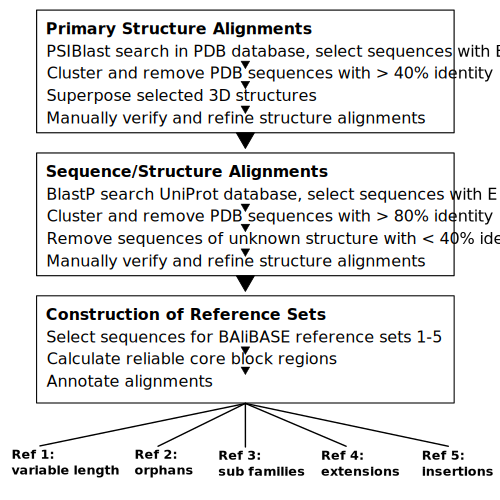
\includegraphics[width=0.5\textwidth]{./images/balibase.png}
	\caption{Flow chart showing the semi automatic process used to establish the reference sets TODO cite self}
	\label{fig:balibase}
\end{wrapfigure}

The third version of the \bb benchmark protein alignment database has been released in 2005 and is widely employed for the comparison of multiple alignment programs \cite{thompson2005balibase, Russell2016}. It is constructed in a semi automatic process as shown in \cref{fig:balibase} and suitable to evaluate global and local alignment programs. The database is split into 5 reference sets with different characteristics representing distinctive multiple alignment problems. \\
It is divided into:



\begin{itemize}
	\item reference set 1 subset V1, for which any two sequences share <20\% identity and no internal insertions over 35 residues long
	\item reference set 1 subset V2, consisting of families with at least four equidistant sequences for which any two sequences share 20-40\% identity and no large insertions
	\item reference set 2, for which all sequences share >40\% identity and at least one 3D structure is known. Additionally an "Orphan" sequence with <20\% identity is chosen per family
	\item for reference set 3, all sequences in the same subfamily have >40\% identity, whereas sequences from different subfamilies share <20\% identity
	\item for reference sets 4 and 5, every sequence shares at least 20\% with one other sequence, including sequences with large N/C-terminal extensions (ref 4) or internal insertions (ref 5)
\end{itemize}

\subsection{Core blocks}

Evaluating and comparing alignment programs is a difficult problem due to the uncertainty of supposedly "real" alignments of actual sequences. The \bb database  marks alignment columns which can be reliably aligned as so called "core blocks". These core blocks are calculated and manually verified, making up 19\% of the full length sequences which are used in the evaluation of \textit{spam-align} \cite{thompson2005balibase}.

%\begin{itemize}
%	\item what are core blocks?
%	\item how are they determined and validated?
%\end{itemize}

\begin{figure}[h]
	\centering
	\includegraphics[width=0.8\textwidth]{./images/balibase-web.png}
	\caption{\bb web interface. Black columns indicate core blocks. \href{www.lbgi.fr/wscoperr?Balibase&FileMoi&macsimHtml&BB20006}{lbgi.fr}}
	\label{}
\end{figure}


\section{Sum-of-pairs and column score}
Comparing the alignment output of different methods can be done by computing the sum-of-pairs and column scores.\\
Given a test alignment $A_t$ and a reference alignment $A_r$ with $M$ sequences and $N_t, N_r$ columns respectively, the sum-of-pairs and column score is defined according to Thompson et al. \cite{thompson1999comprehensive}.

\begin{mydef}[Sum-of-pairs score]
	The sum of pairs score is the ratio of correctly aligned individual residues. Formally it is defined as:
	\begin{align*}
		p_{ijk} &= \begin{cases}
		1 \text{ if residues $A_{t{_ij}}$ and $A_{t_{ik}}$ \textbf{are} aligned in $A_r$}\\
		0 \text{ otherwise}
		\end{cases} \\
		S_i &= \sum_{j=1}^{M} \sum_{k=i+1}^{M} p_{ijk} \\
		SPS &= \frac{\sum_{i=1}^{N_t} S_i} {\sum_{i=1}^{N_r} S_{r_i}}
 	\end{align*}
 	with $S_{r_i}$ being the number of correctly aligned residues in the reference.
\end{mydef}

\begin{mydef}[Column score]
	The column score is the ratio of correctly aligned columns. 
	\begin{align*}
	C_i &= \begin{cases}
	1 \text{ if all the residues in the i-th column are aligned correctly}\\
	0 \text{ otherwise}
	\end{cases} \\
	CS &= \frac{\sum_{i=1}^{N_t} C_i}{N_r}
	\end{align*}
\end{mydef}
Note that $C_i = 1$ only if all the residues in the $i$-th column are aligned correctly and no residue belonging to this column is part of another one. For this reason, the numerator is smaller or equal to the denominator.\\
The definition of the column score is slightly different than that provided by the authors of \bb \cite{thompson1999comprehensive} but resembles the actual implementation in the included BaliScore tool and its reimplementation provided with this thesis.\\
These scores are only calculated for the core blocks of the \bb alignments, meaning that for the following evaluation $A_t$ is an alignment over the full sequences, while $A_r$ contains only the aligned residues inside the core blocks.

\section{Evaluated programs}


\subsection{Mafft}
Additionally to \textit{Dialign2.2} and \textit{spam-align} the widely used multiple alignment program \textit{MAFFT} (version 7) is evaluated. It employs a progressive alignment strategy 

\begin{itemize}
	\item progressive alignment
	\item guide tree from all pairwise alignments
\end{itemize}

\subsection{Dialign}

\subsection{Spam}

\section{Results}

    \myemptypage


    \chapter{Conclusion}

\subsection{Further work}
    \myemptypage

    %--- references ---
    \bibliographystyle{IEEEtran}
    \bibliography{content/references}
    \addcontentsline{toc}{chapter}{\bibname}
    \myemptypage

    %--- appendix ---
    \begin{appendix}
        \input{content/appendix_a}
        \myemptypage
    \end{appendix}
    
\end{document}